\usetikzlibrary{arrows,calc}

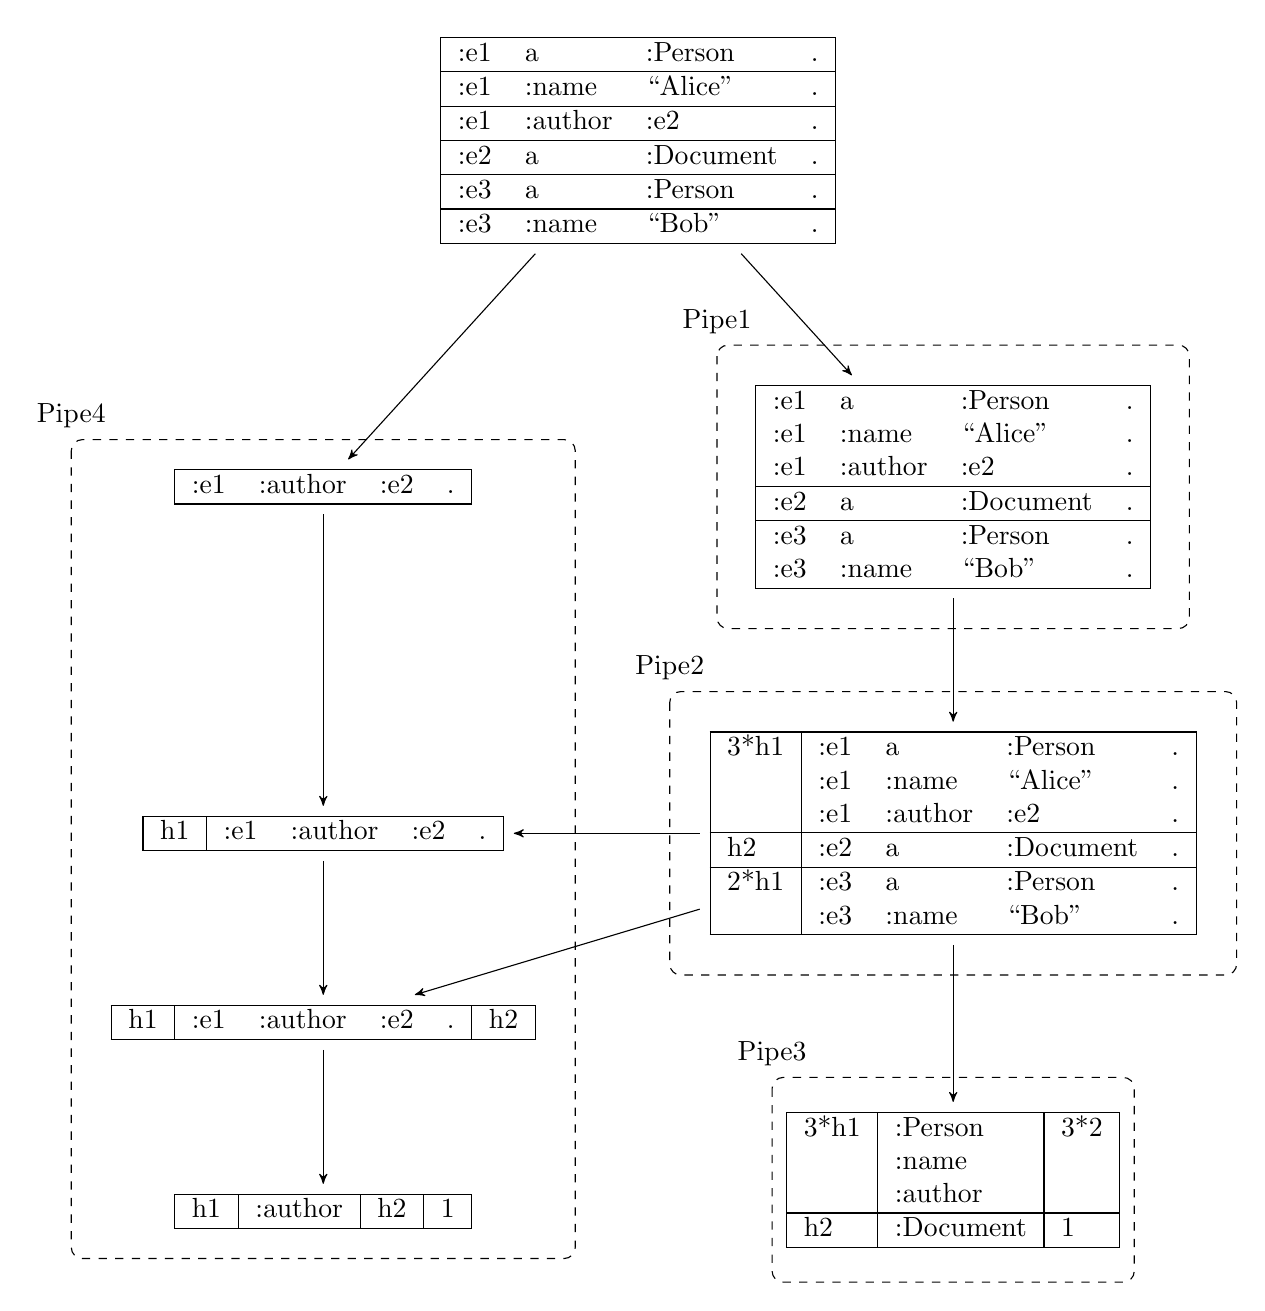
\begin{tikzpicture}[->,>=stealth',node distance=4.4cm]
\node (data) {
\begin{tabular}{|llll|}
\hline
:e1 & a & :Person & . \\
\hline
:e1 & :name &``Alice'' & . \\
\hline
:e1 & :author & :e2 & . \\
\hline
:e2 & a & :Document & . \\
\hline
:e3 & a & :Person & . \\
\hline
:e3 & :name & ``Bob'' & . \\
\hline
\end{tabular}
};

\node[below of = data,xshift=4cm] (edesc) {
\begin{tabular}{|llll|}
\hline
:e1 & a & :Person & . \\
:e1 & :name &``Alice'' & . \\
:e1 & :author & :e2 & . \\
\hline
:e2 & a & :Document & . \\
\hline
:e3 & a & :Person & . \\
:e3 & :name & ``Bob'' & . \\
\hline
\end{tabular}
};

\node[below of = edesc] (gsv) {
\begin{tabular}{|l|llll|}
\hline
\multirow{3}{*}{h1} & :e1 & a & :Person & . \\
& :e1 & :name &``Alice'' & . \\
& :e1 & :author & :e2 & . \\
\hline
h2 & :e2 & a & :Document & . \\
\hline
\multirow{2}{*}{h1} & :e3 & a & :Person & . \\
& :e3 & :name & ``Bob'' & . \\
\hline
\end{tabular}
};

\node[below of = data,xshift=-4cm] (filtered) {
\begin{tabular}{|llll|}
\hline
:e1 & :author & :e2 & . \\
\hline
\end{tabular}
};

\node[below of = filtered] (join1) {
\begin{tabular}{|l|llll|}
\hline
h1 &:e1 & :author & :e2 & . \\
\hline
\end{tabular}
};

\node[below of = join1,yshift=2cm] (join2) {
\begin{tabular}{|l|llll|l|}
\hline
h1 & :e1 & :author & :e2 & . & h2 \\
\hline
\end{tabular}
};

\node[below of = join2,yshift=2cm] (relagg) {
	\begin{tabular}{|l|l|l|l|}
	\hline
	h1 & :author & h2 & 1\\
	\hline
	\end{tabular}
};

\node[below of = gsv] (attagg) {
\begin{tabular}{|l|l|l|}
\hline
\multirow{3}{*}{h1} & :Person & \multirow{3}{*}{2} \\
 & :name & \\
 & :author & \\
\hline
h2 & :Document & 1 \\
\hline
\end{tabular}
};

\coordinate (p1x) at ($ (filtered) + (-3.2,.6) $);
\coordinate (p1y) at ($ (relagg) + (3.2,-.6) $);
\draw[rounded corners,dashed]  (p1x) node[yshift=.3cm] {Pipe4} rectangle (p1y);

\coordinate (p2x) at ($ (edesc) + (-3,1.8) $);
\coordinate (p2y) at ($ (edesc) + (3,-1.8) $);
\draw[rounded corners,dashed]  (p2x) node[yshift=.3cm] {Pipe1} rectangle (p2y);

\coordinate (p3x) at ($ (gsv) + (-3.6,1.8) $);
\coordinate (p3y) at ($ (gsv) + (3.6,-1.8) $);
\draw[rounded corners,dashed]  (p3x) node[yshift=.3cm] {Pipe2} rectangle (p3y);

\coordinate (p4x) at ($ (attagg) + (-2.3,1.3) $);
\coordinate (p4y) at ($ (attagg) + (2.3,-1.3) $);
\draw[rounded corners,dashed]  (p4x) node[yshift=.3cm] {Pipe3} rectangle (p4y);

\path
(data) edge (edesc)
(data) edge (filtered)
(filtered) edge (join1)
(edesc) edge (gsv)
(gsv) edge (join1)
(join1) edge (join2)
(gsv) edge (join2)
(join2) edge (relagg)
(gsv) edge (attagg)
;
\end{tikzpicture}